\chapter{Experiements}
%\section{Experiments}

\section{Performance measurement}
Before we go further and present the experiments and results it is necessary to
introduce some additional terms. Such as metrics to measure their performance.

\paragraph{Mean squared error (MSE)} is an error measurement that
describes the error between an given or measured reference signal $\vec{x}$
and and the reconstruction(noisy approximation) $\vec{\tilde{x}}$ of it.
Mathematically it is defined as the average of the squared error between two
signals.
%The mean squared error is defined as:
\begin{equation*}
 MSE = \frac{1}{n} \sum_{i=0}^{n} \left( {\lVert x_i -
\tilde{x}_i\rVert^{2}}\right)
\end{equation*}
We primarily use it for testing dictionary learning convergence and as a
sub term for the measurement described in the next paragraph.

\paragraph{Peak signal-to-noise ration (PSNR)} describes the ratio between the
noise affecting a signal and the maximum possible signal amplitude. It is
expressed in a logarithmic decibel scale.
\begin{equation*}
 PSNR = 20 \cdot \log_{10} \left(\frac{MAX}{\sqrt{MSE}}\right)
\end{equation*}
Where $MAX$ is the maximum possible value of our signal. For an 8-bit
image it would be 255. For a 32-bit normalized image it would be 1. And $MSE$ is
the mean squared error between a reference signal and its reconstruction. The
PSNR is undefined for zero noise.

The PSNR is primarily used for comparison of the reconstruction quality of
lossy compression algorithms. Typical values for a lossy reconstruction lie in
a range between 30dB and
50dB.\footnote{\url{http://en.wikipedia.org/wiki/Peak_signal-to-noise_ratio}}
%e.g. relevant for de-noise

\paragraph{Bits per pixel (bpp)} 
For the comparison of compression ratio of images another well known practice is
to measure the required \emph{bits per pixel} short bpp. The bbp are calculated
by dividing the raw image data by the image's dimensions. For example an
uncompressed RGB color image with 8-bit of color depth requires 24-bits per
pixel, respectively a gray scale image with 8-bit for a single channel requires
8-bits. While compression algorithms are able to encode multiple pixels with few
coefficient leading to much lower bpp rates.
Looking at other well known compression algorithms such as JPEG or
JPEG 2000 a common ratio is about $\sim1.8$ bits-per-pixel for average
quality compression( JPEG quality of 50) of an natural image. 

\Todo{example image?, lower bit rates, Lewicki estimate for sparse coding}

\paragraph{Test data}
In addition to the introduced metrics it is common practice to use some image
sets to compare test results of the different algorithms and parameter
configurations. As the dictionaries are specificaly trained for
reconstruction of the data in the training sets
(\prettyref{fig:database_images}) it is mandatory to also use
these image to test the reconstruction and
compression quality. 
\begin{figure}[h]
\centering
% \subfloat{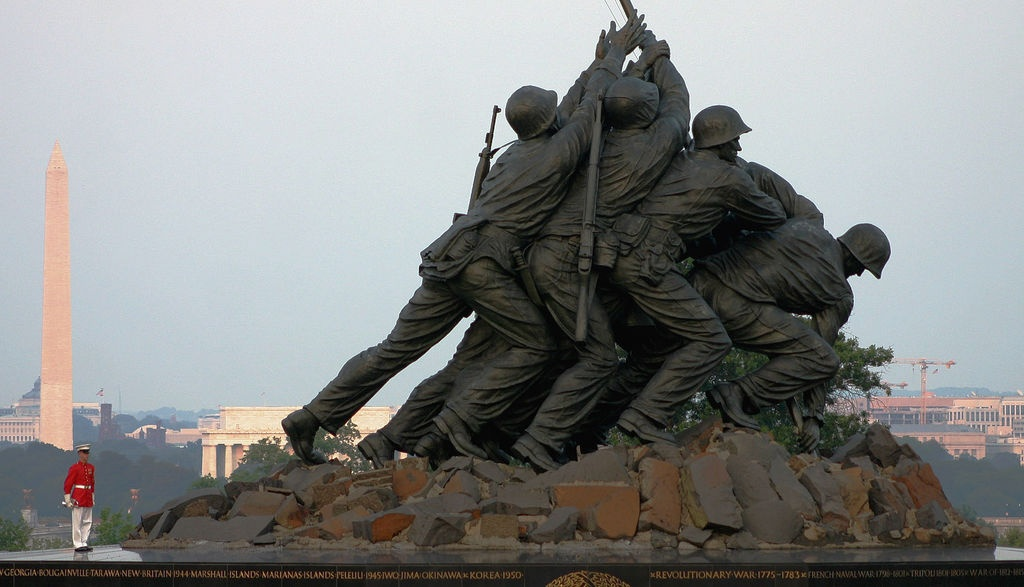
\includegraphics[width = 0.3\textwidth]{images/28979823.jpg}}
% \hspace{5mm}
% \subfloat{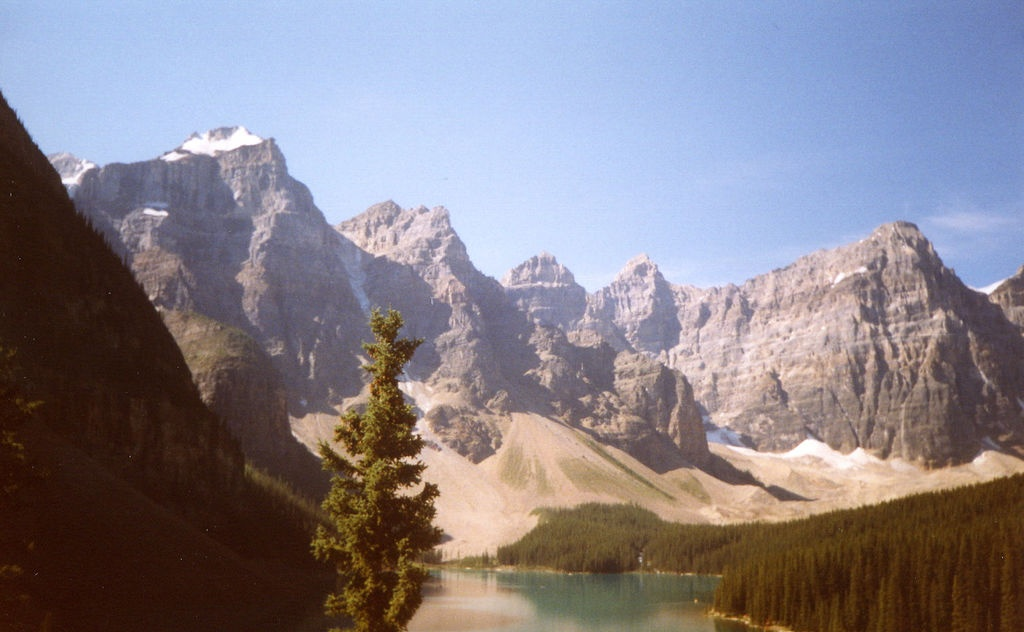
\includegraphics[width = 0.3\textwidth]{images/29018694.jpg}}
% \hspace{5mm}
% \subfloat{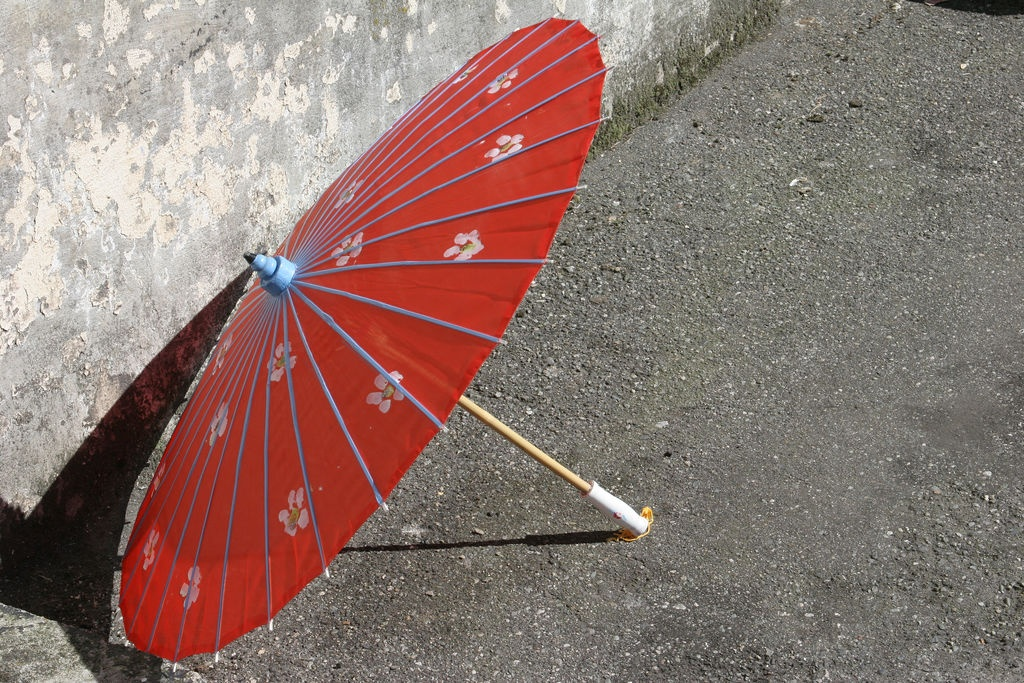
\includegraphics[width = 0.3\textwidth]{images/28874882.jpg}}
% \hspace{5mm}
\subfloat{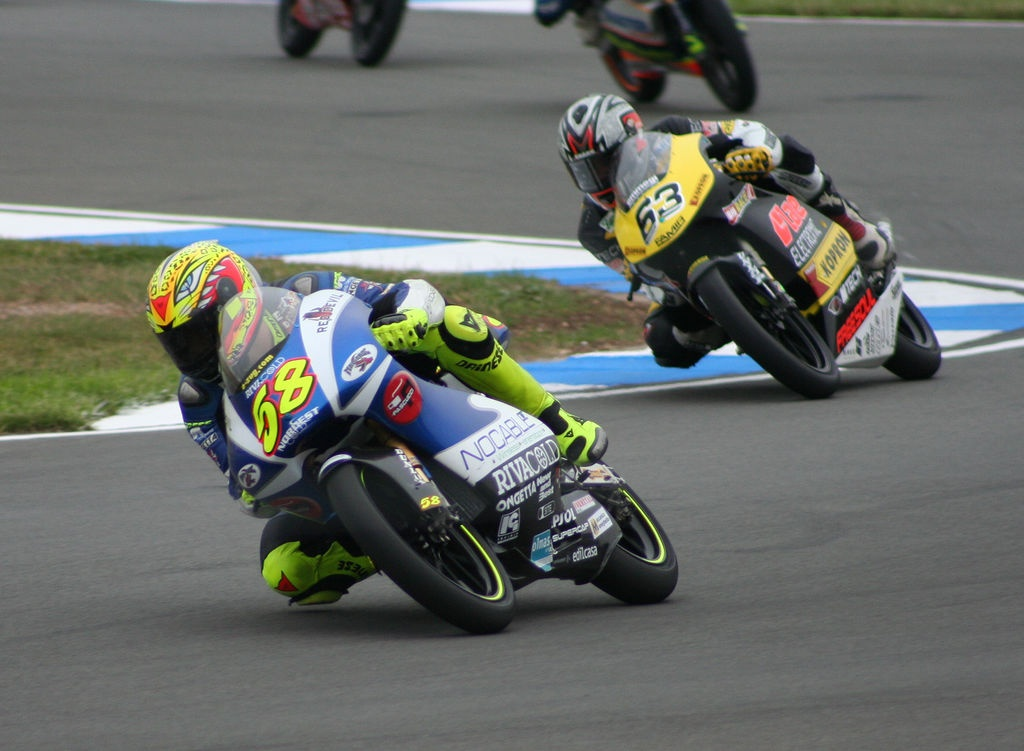
\includegraphics[width = 0.3\textwidth]{images/28803842.jpg}}
\hspace{5mm}
\subfloat{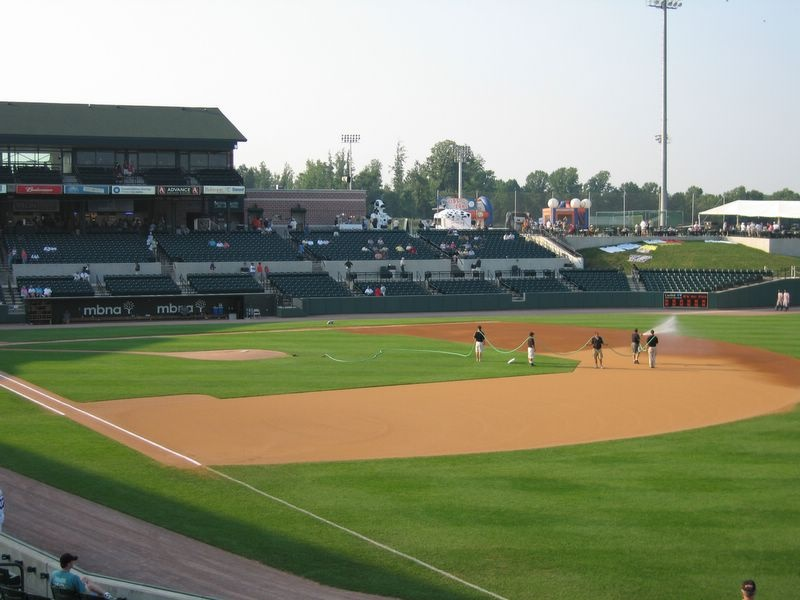
\includegraphics[width = 0.3\textwidth]{images/28894495.jpg}}
\hspace{5mm}
\subfloat{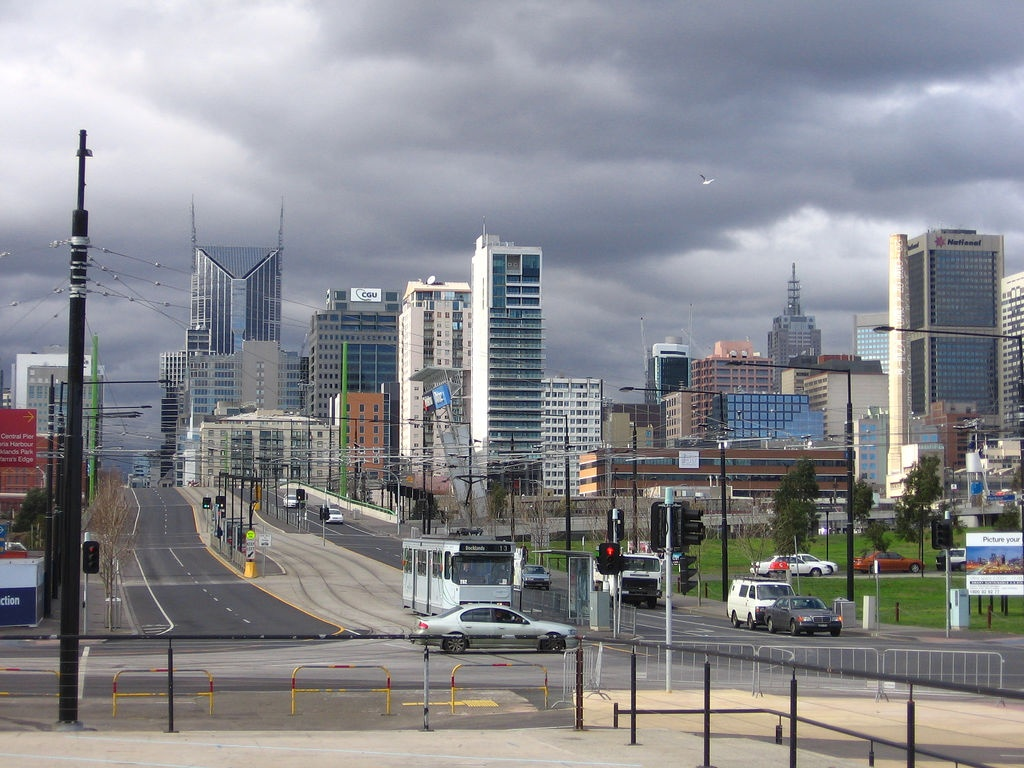
\includegraphics[width = 0.3\textwidth]{images/28952841.jpg}}
\hspace{5mm}
\subfloat{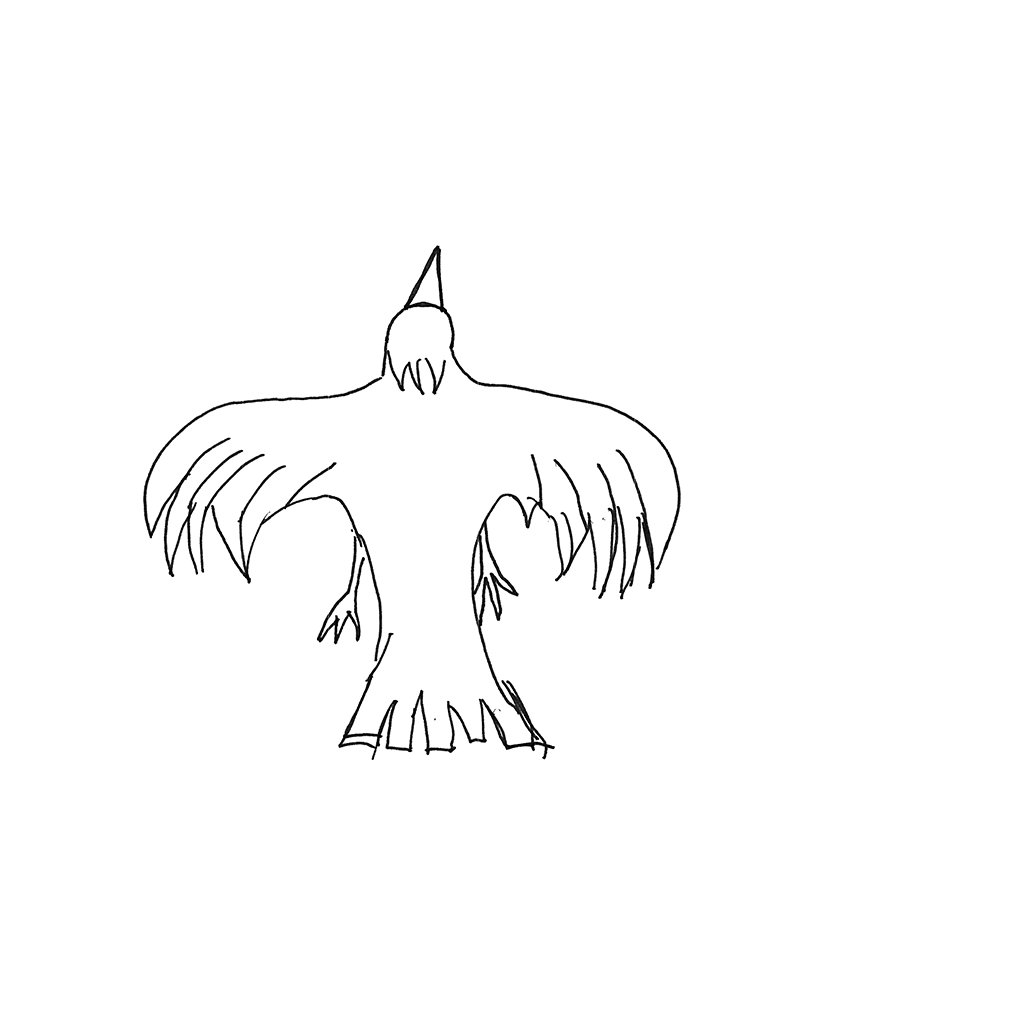
\includegraphics[width = 0.3\textwidth]{images/sketch1.jpg}}
\hspace{5mm}
\subfloat{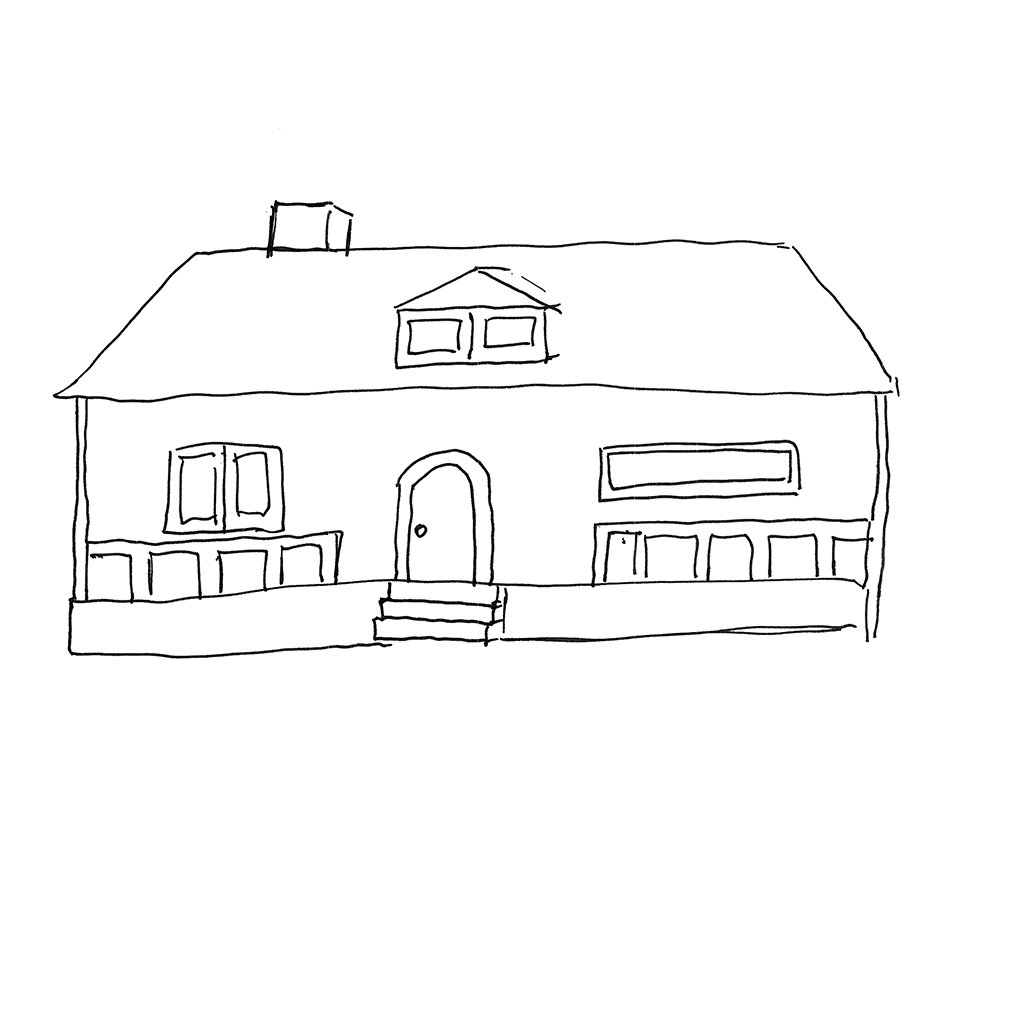
\includegraphics[width = 0.3\textwidth]{images/sketch2.jpg}}
\hspace{5mm}
\subfloat{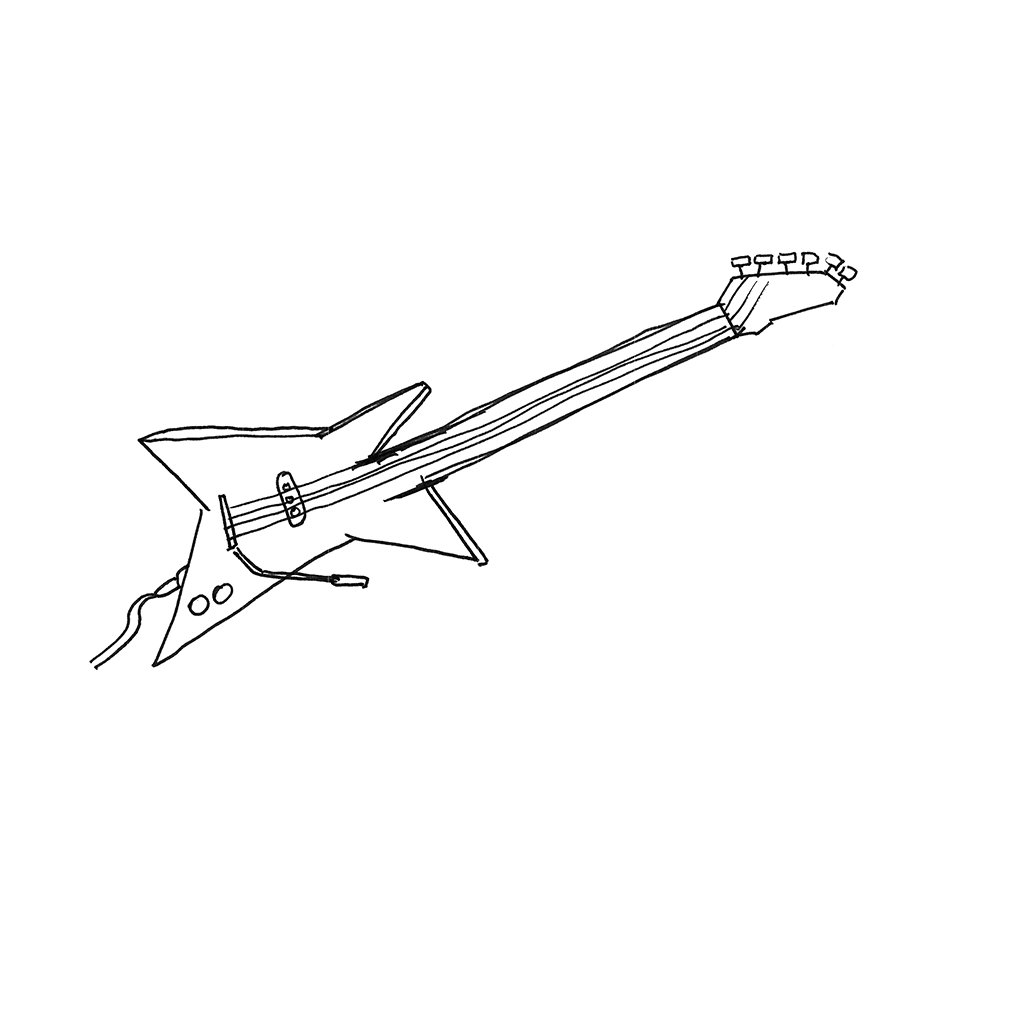
\includegraphics[width = 0.3\textwidth]{images/sketch3.jpg}}
\hspace{5mm}
\caption{example images from natural image and sketch training sets}
\label{fig:database_images}
\end{figure}


In addition to this we want to know how good the dictionaries can reconstruct
and compress images outside of the database respectifly the training set. For
those comparisons we use a selection (\prettyref{fig:USC-SIPI}) from a
well known set of standard test images from the \emph{USC-SIPI Image
Database}\footnote{\url{http://sipi.usc.edu/database/}}
(\prettyref{fig:USC-SIPI}). 
%Including pictures such as Lena, Mandrill and Peppers.
\begin{figure}[H]
\centering
%\subfloat{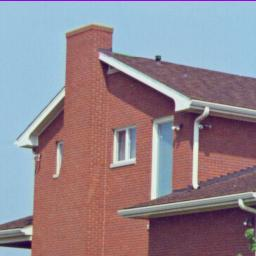
\includegraphics[width = 0.3\textwidth]{images/4_1_05.jpg}}
%\hspace{5mm}
\subfloat{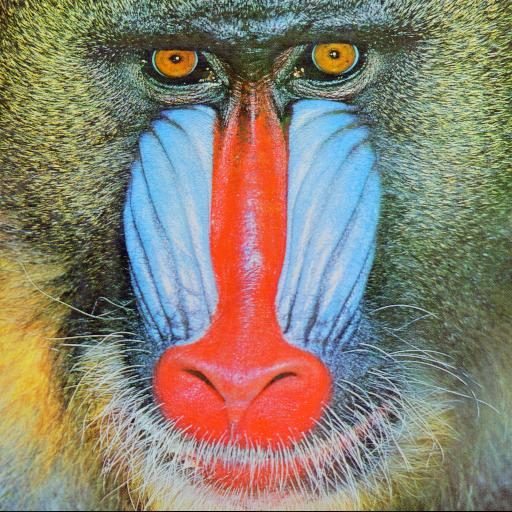
\includegraphics[width = 0.3\textwidth]{images/4_2_03.jpg}}
\hspace{5mm}
\subfloat{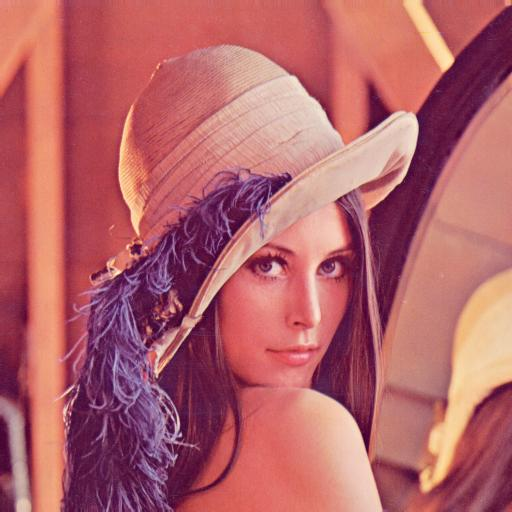
\includegraphics[width = 0.3\textwidth]{images/4_2_04.jpg}}
\hspace{5mm}
%\subfloat{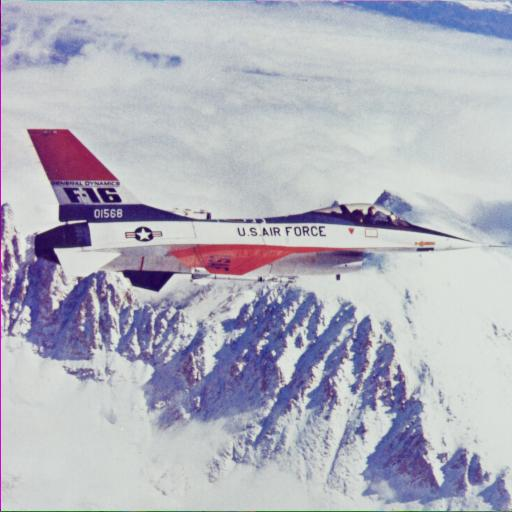
\includegraphics[width = 0.3\textwidth]{images/4_2_05.jpg}}
%\hspace{5mm}
%\subfloat{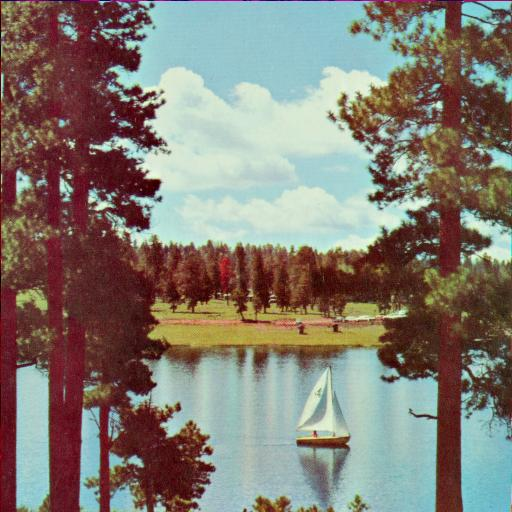
\includegraphics[width = 0.3\textwidth]{images/4_2_06.jpg}}
%\hspace{5mm}
\subfloat{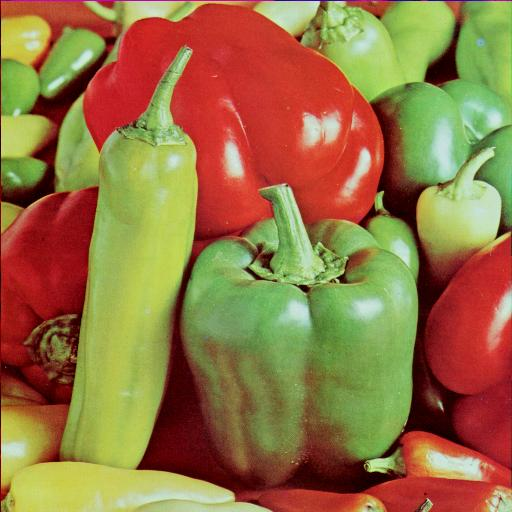
\includegraphics[width = 0.3\textwidth]{images/4_2_07.jpg}}
\caption{test images from USC-SIPI Image Database}
\label{fig:USC-SIPI}
\end{figure}


\section{Hardware setup} 
Computations were made on a cluster of 100 clients. Each 
configured with a AMD Athlon 64 X2 (2x2.6GHz) and 3GB RAM.
The operating system running Debian Linux with 32-bit kernel. 

\section{Learning parameters}
At first we needed to find good start settings for experiments with large set of
different samples and big dictionaries. This involves the
avarage number of learning coefficients, block size, sample selection strategy
and mini-batch size.

Mairal et al. already propose some learning parameters for their online
learning algorithm. But as most other they only learn dictionaries with
a small redundancy of up to four times and compact training sets with 100,000
to 1,000,000 samples that get randomly evaluated until convergence of the
dictionary.

We wanted to find start settings for experiments with large sets of
different samples with no reevaluation of the samples and dictionaries
with much bigger redundancy of 10 to 50 times.

An average of 10 learning coefficients is suggested as it produces enougth
sparseness and leads to good and fast convergence of the dictionaries.
We tested if this also applies to big numbers of samples and bigger
dictionaries. We compared the reconstruction quality dependency on the average
number of coefficients in the learning process. Both OMP
(\prettyref{fig:coeffsOMP}) and LARS-Lasso (\prettyref{fig:coeffsLasso}) runs
were made.
\begin{figure}[h]
\centering
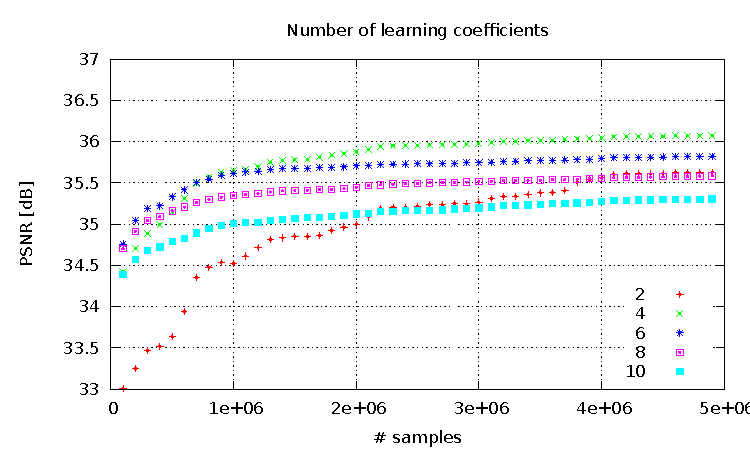
\includegraphics[width = 0.8\textwidth]{../tests/results/old/coeffsConverg.pdf}
\caption{reconstruction quality for different training coefficients (OMP)}
\label{fig:coeffsOMP}
\end{figure}
\begin{figure}[h]
\centering
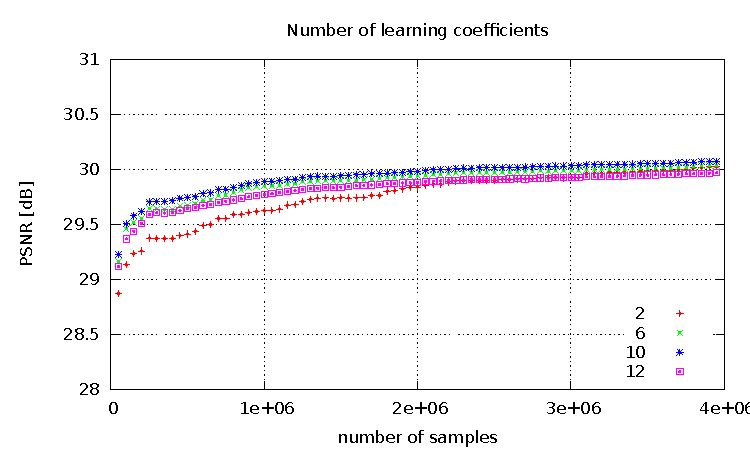
\includegraphics[width = 0.8\textwidth]{../tests/results/coeffsConverg.pdf}
\caption{reconstruction quality for different training coefficients (LARS)}
\label{fig:coeffsLasso}
\end{figure}

Convergence of quality of different number of learning coefficients.
With high number of learning coefficents convergence is reached faster than
with a low number of coefficents but for large dicts fewer coefficents lead to
better reconstruction quality with larger training sets.


Afterwards compared the reconstruction quality dependency on block size in the
learning process.

\begin{figure}[h]
\centering
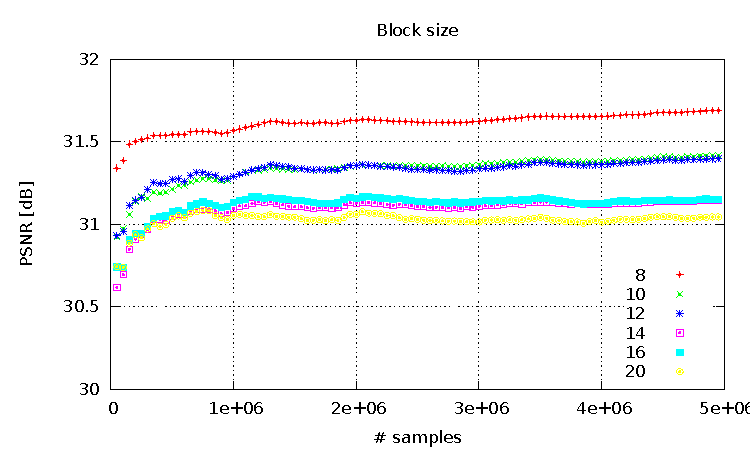
\includegraphics[width =
0.8\textwidth]{../tests/results/old/blockSizeConverg.pdf}
\caption{reconstruction quality for different block sizes}
\label{fig:dict size}
\end{figure}

Convergence of quality of different block sizes.
But large blocks 

\subsection{Structure}
At then end we want to know how the structure of the learned atoms from natural
images looks like. Do they resemble known structures from designed dictionaries?
How do these learned structures change with the block size of the atoms?
What structure show samples from other groups of images?

Appearance 
Learn basis similar to DCT and wavelets/bandelets(time and freq locality) with
increasing block size. Use to verify if it is a jpeg image?
Similar to natural images.
compression dicts
Dictionaries to universal ... improved results to DCT .. but varying with field
of application. possible no universal solution but a good way for better
understanding of the key elements
  four major types of elements
  gradient, checkerboard (low color more b/w), spot, edge
Better understanding the selection strategies of the algorithm and their
meaning for perceptional image quality. And evolution of the structure of
learned dictionaries. 

\begin{figure}[H]
\centering
\subfloat{
\includegraphics[width = 0.3\textwidth]{images/gradient.png}}
\hspace{5mm}
\subfloat{
\includegraphics[width = 0.3\textwidth]{images/checkerboard.png}}
\hspace{5mm}
\subfloat{
\includegraphics[width = 0.3\textwidth]{images/spot.png}}
\hspace{5mm}
\subfloat{
\includegraphics[width = 0.3\textwidth]{images/edges.png}}
\hspace{5mm}
\subfloat{
\includegraphics[width = 0.3\textwidth]{images/wavelet.png}}
\caption{image from database}
\label{fig:USC-SIPI}
\end{figure}

For the small training sets Mairal et al. suggest mini-batch size of two to four
times the size of the the dictionary. No significant oberservations were made
and we stuck to these sizes. 


\section{Dictionary size}
After we found good settings to learn from large sets of different images we
wanted to know how big we can make the dictionaries and still profit from them.
And if reconstruction quality increases with dictionaries size and when
convergence is reached.

\begin{figure}[h]
\centering
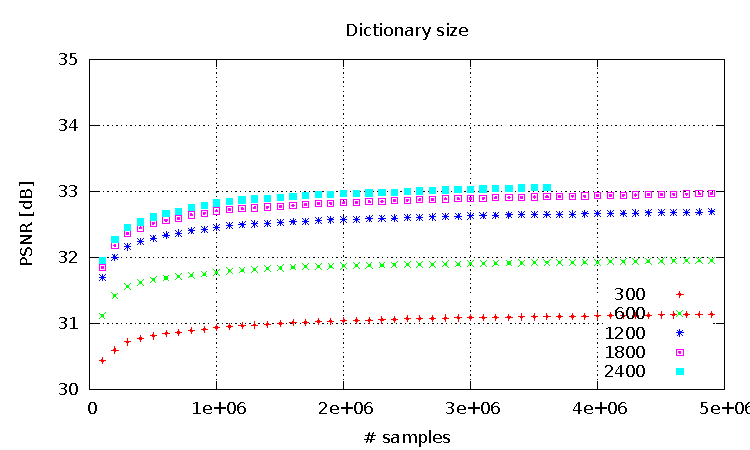
\includegraphics[width = 0.8\textwidth]{../tests/results/old/dictSizeOMP.pdf}
\caption{reconstruction quality for different dictionary sizes (OMP)}
\label{fig:dictSizeOMP}
\end{figure}


\begin{figure}[h]
\centering
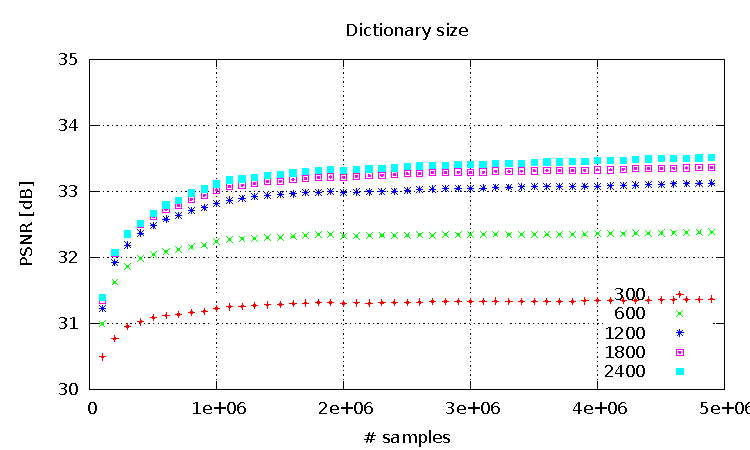
\includegraphics[width = 0.8\textwidth]{../tests/results/old/dictSizeLasso.pdf}
\caption{reconstruction quality for different dictionary sizes (Lasso)}
\label{fig:dict size}
\end{figure}

In addition we compared the cluster approach performs in
comparisons to a dictionary learned in single. Each client in the cluster
calculated batches of 100--10,000 images based on the
size of the training sets.




\section{Compression}
Besides the ability of learned dictionaries 
we used the simple compression algorithm from \prettyref{sec:compression} .
and compared it to a collection of JPEG and JPEG 2000 compressed images with the
same file size. The objective was to investigate the compression ratio and if
the extra amount of index data is a big hit on the overall load.
One benefit of the learned dictionary approach that plays well in our
hands is the ability to to learn and use specific dictionaries for each group of
images. We tested this by learning a dictionary from a set of sketch images and
used it to compress sketches. A domain in which the JPEG compression performs
bad.

Compression
For the short time available the results show promising results in visual
quality but still lack ...

Using LARS-Lasso for training generates a good dictionary for LARS and OMP. 
\Todo{ Training with OMP leads to a dictionary more with a lot of noise that
leads better coding results when using OMP.}


% Difference in the selection strategy.
% Very noisy vs. smooth. 
% How this different selection strategies affect the learning step will be
% presented in the next section.
\subsection{Natural images}

\begin{figure}[h]
\centering
\subfloat{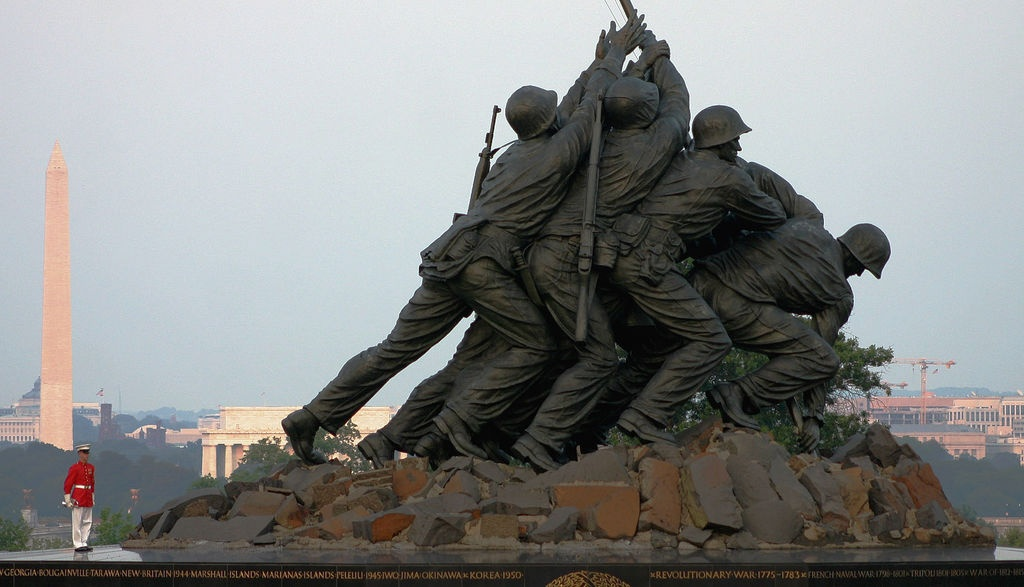
\includegraphics[width = 0.3\textwidth]{images/28979823.jpg}}
\hspace{5mm}
\subfloat{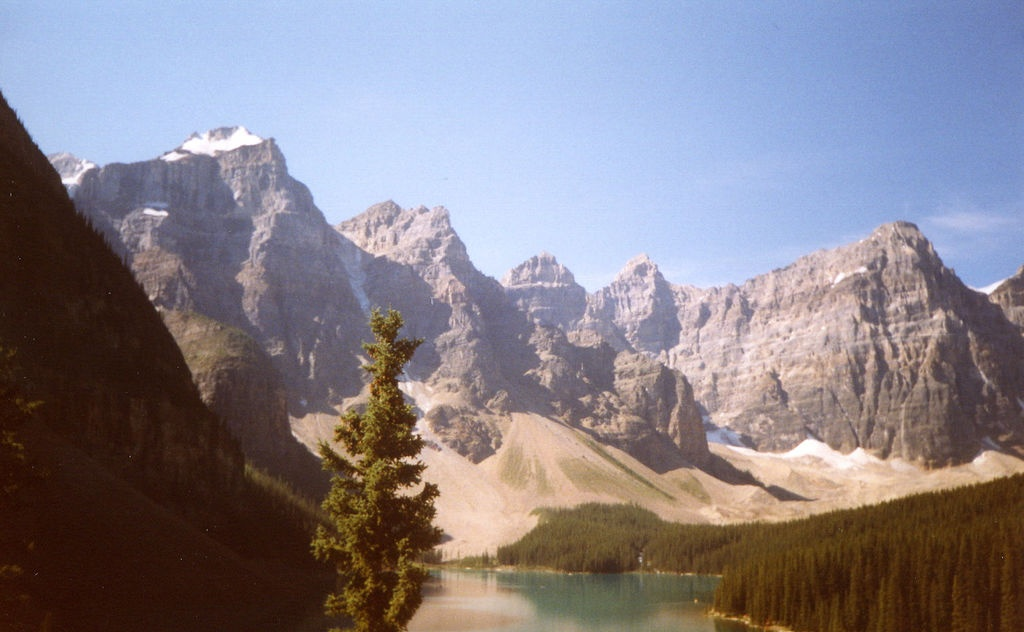
\includegraphics[width = 0.3\textwidth]{images/29018694.jpg}}
\hspace{5mm}
\subfloat{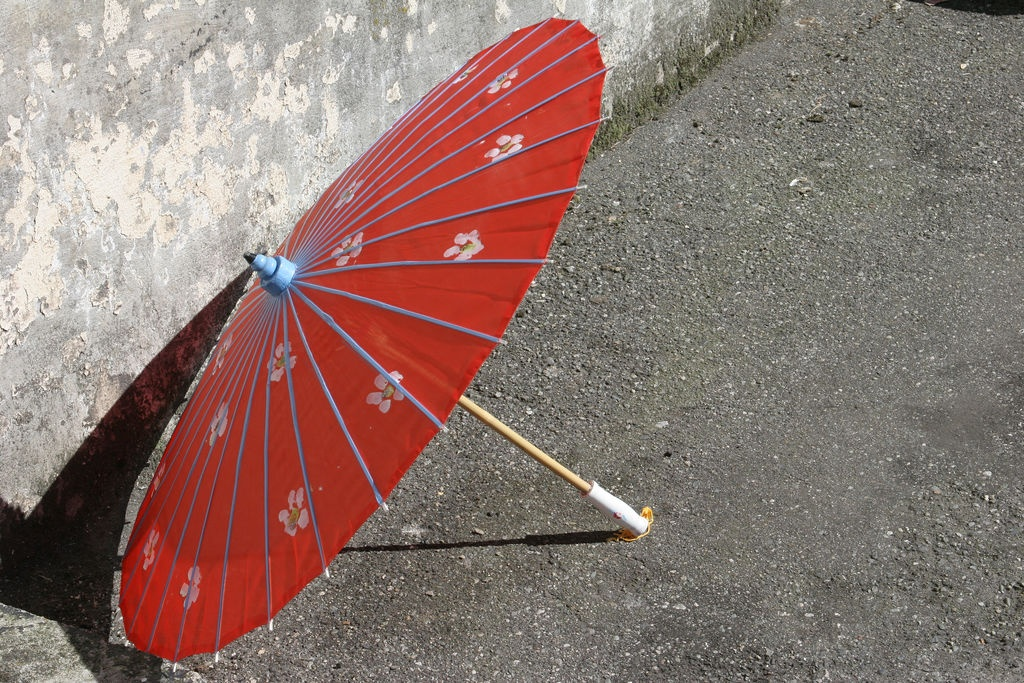
\includegraphics[width = 0.3\textwidth]{images/28874882.jpg}}
\hspace{5mm}
\subfloat{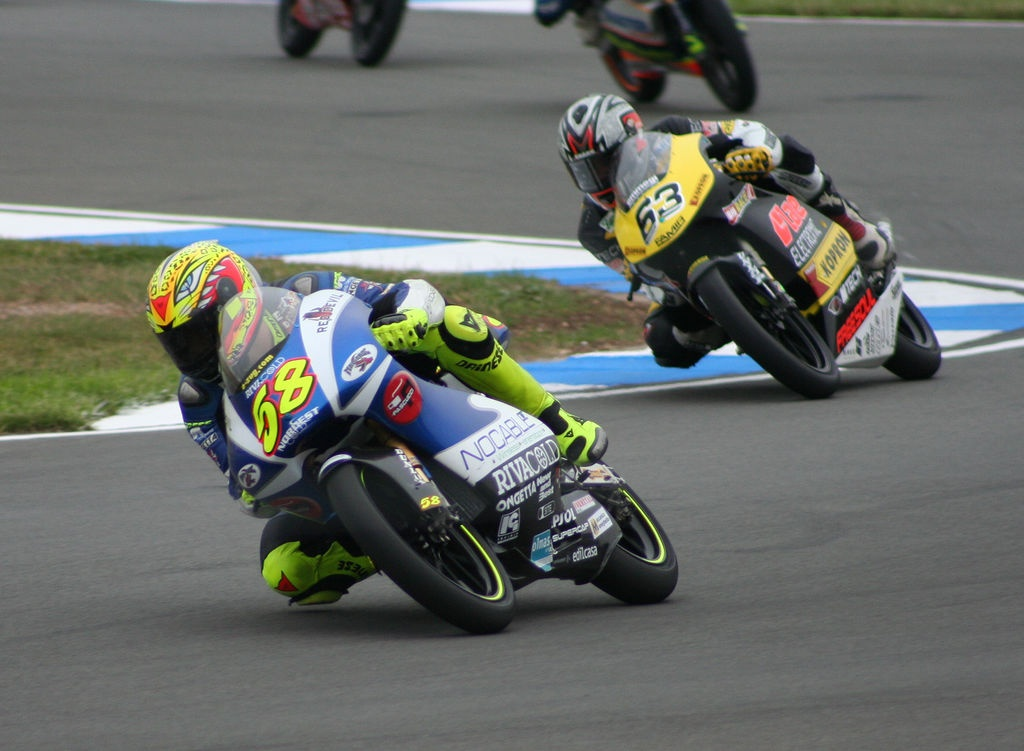
\includegraphics[width = 0.3\textwidth]{images/28803842.jpg}}
\hspace{5mm}
\subfloat{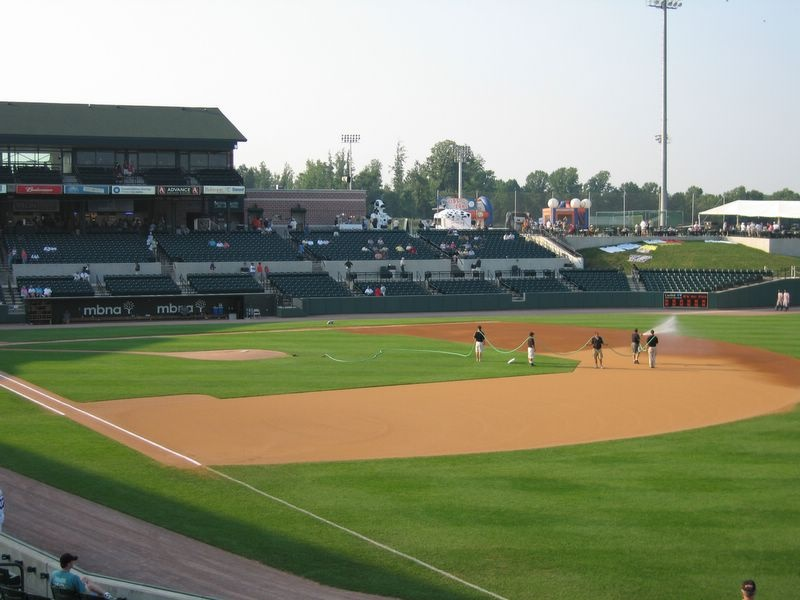
\includegraphics[width = 0.3\textwidth]{images/28894495.jpg}}
\hspace{5mm}
\subfloat{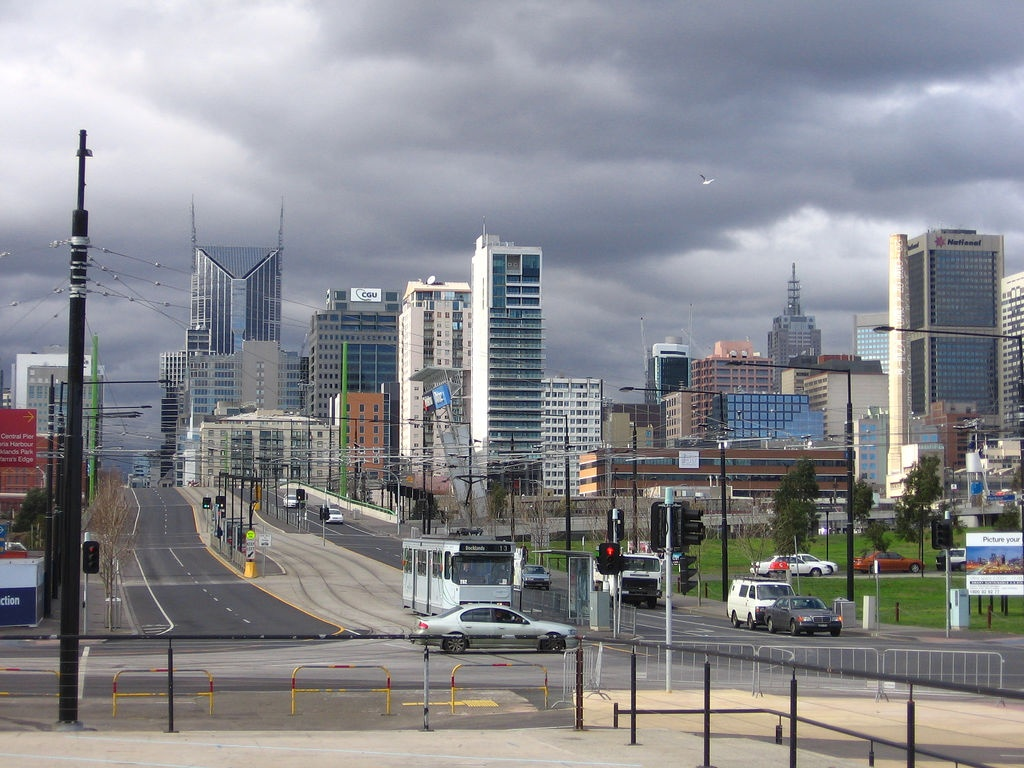
\includegraphics[width = 0.3\textwidth]{images/28952841.jpg}}
\caption{test images from training set}
\label{fig:database_images}
\end{figure}

\begin{table}[H]
%\caption{single vs. cluster}
\centering
\begin{tabular}{| l c | c | c | c|}
\hline\hline
Image & bpp & SPRS & JPEG & JPEG2000 \\
\hline
image 1 & 1.12 & 31.2205 & 32.3289 & 36.613 \\
image 2 & 1.01 & 34.7735 & 35.0671 & 40.3299 \\
image 3 & 1.8  & 29.0597 & 27.2556 & 31.7412 \\
image 4 & 0.74  & 35.9499 & 35.5104 & 39.4195 \\

\hline
\end{tabular}
\end{table}

\begin{figure}[H]
\centering
\subfloat[sprs ]{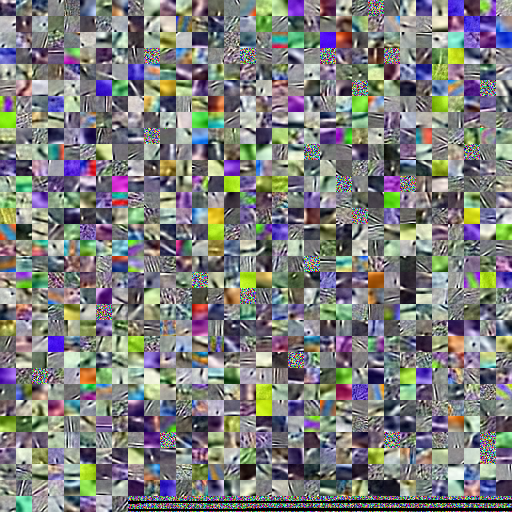
\includegraphics[width =
0.3\textwidth]{images/16_1000_1000_10_lasso.png}}
\hspace{5mm}
\subfloat[JPEG]{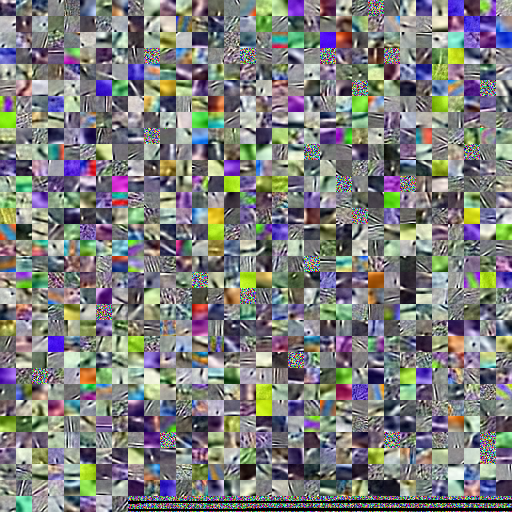
\includegraphics[width =
0.3\textwidth]{images/16_1000_1000_10_lasso.png}}
\hspace{5mm}
\subfloat[JPEG2000]{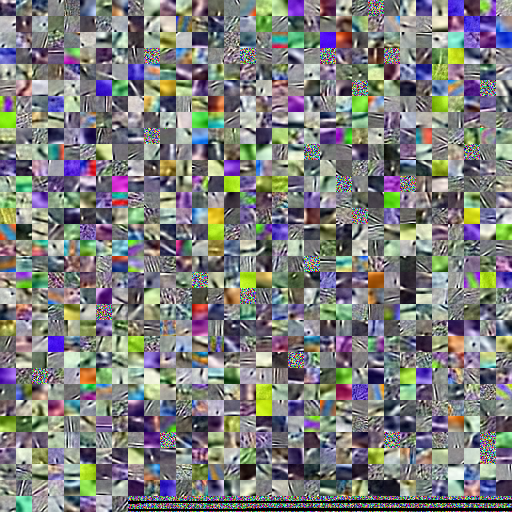
\includegraphics[width =
0.3\textwidth]{images/16_1000_1000_10_lasso.png}}
%\caption{}
%\label{fig:16_1000_lasso}
\end{figure}

\begin{figure}[H]
\centering
\subfloat[sprs]{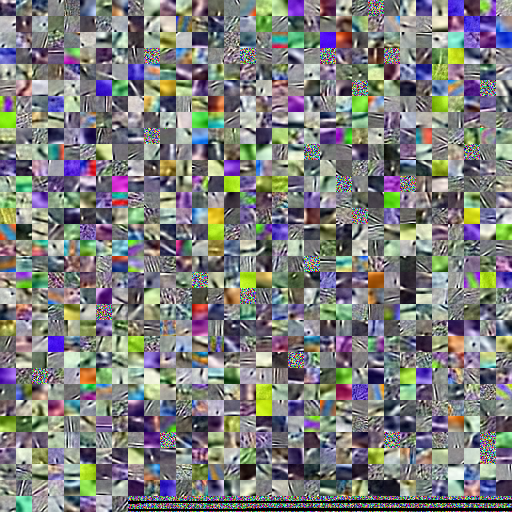
\includegraphics[width =
0.3\textwidth]{images/16_1000_1000_10_lasso.png}}
\hspace{5mm}
\subfloat[JPEG]{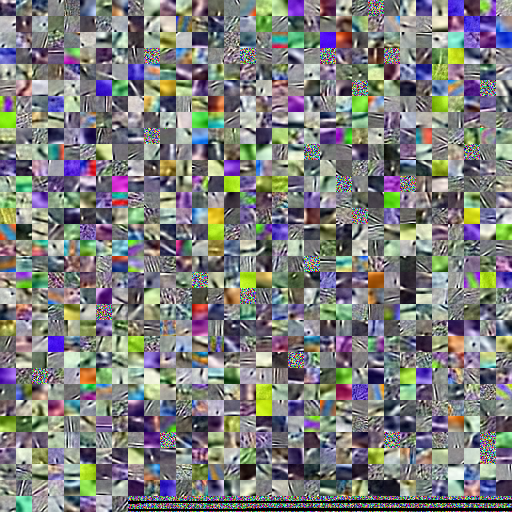
\includegraphics[width =
0.3\textwidth]{images/16_1000_1000_10_lasso.png}}
\hspace{5mm}
\subfloat[JPEG2000]{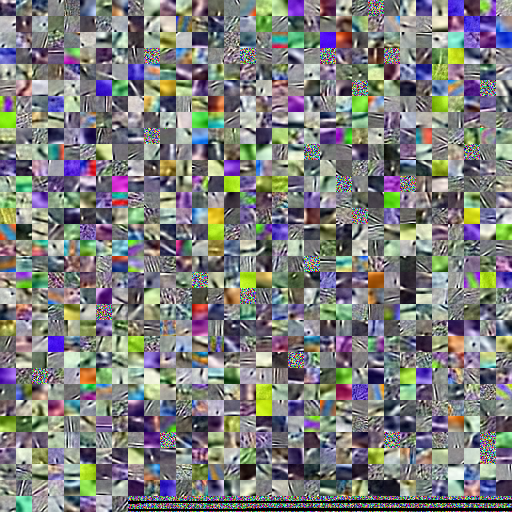
\includegraphics[width =
0.3\textwidth]{images/16_1000_1000_10_lasso.png}}
%\caption{}
%\label{fig:16_1000_lasso}
\end{figure}



\newpage
\subsection{Sketches}

\begin{figure}[h]
\centering
\setcounter{subfigure}{0}
\subfloat[]{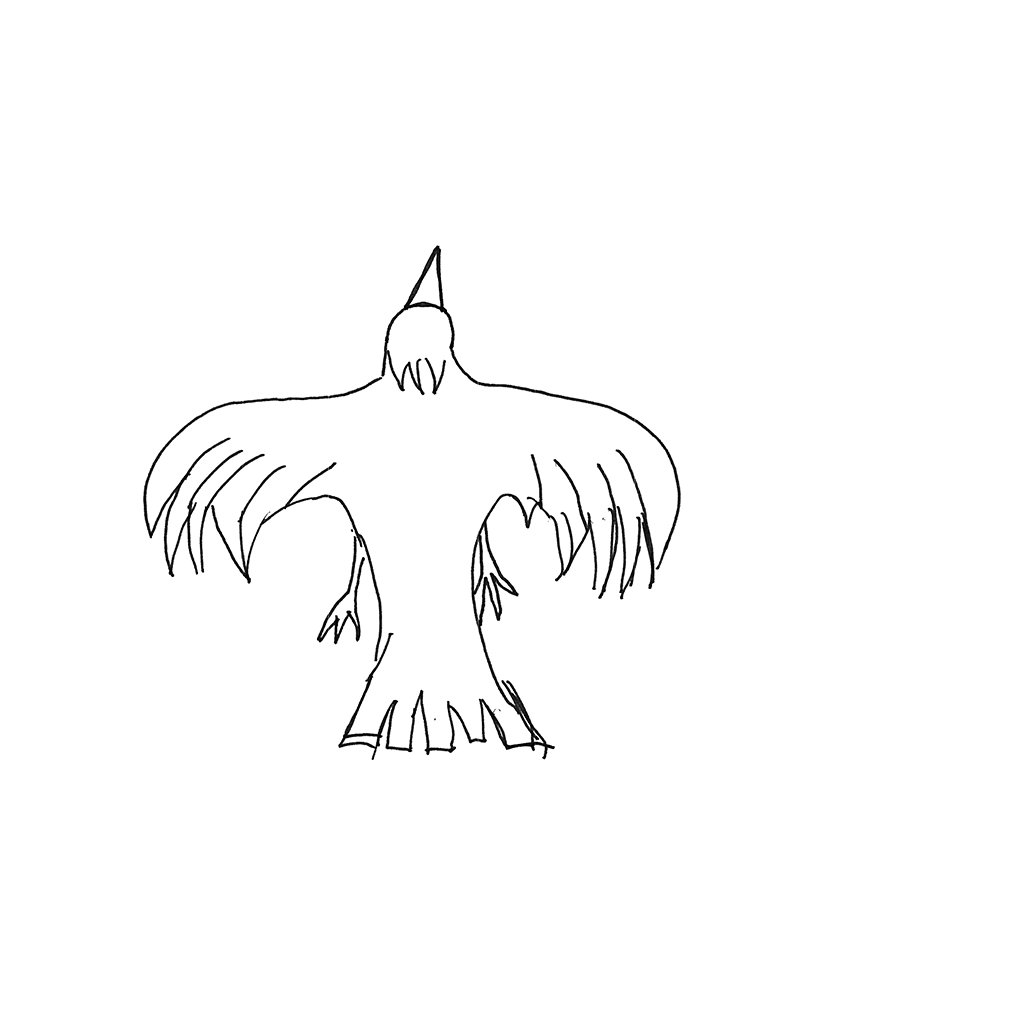
\includegraphics[width =
0.3\textwidth]{images/sketch1.jpg}}
\hspace{5mm}
\subfloat[]{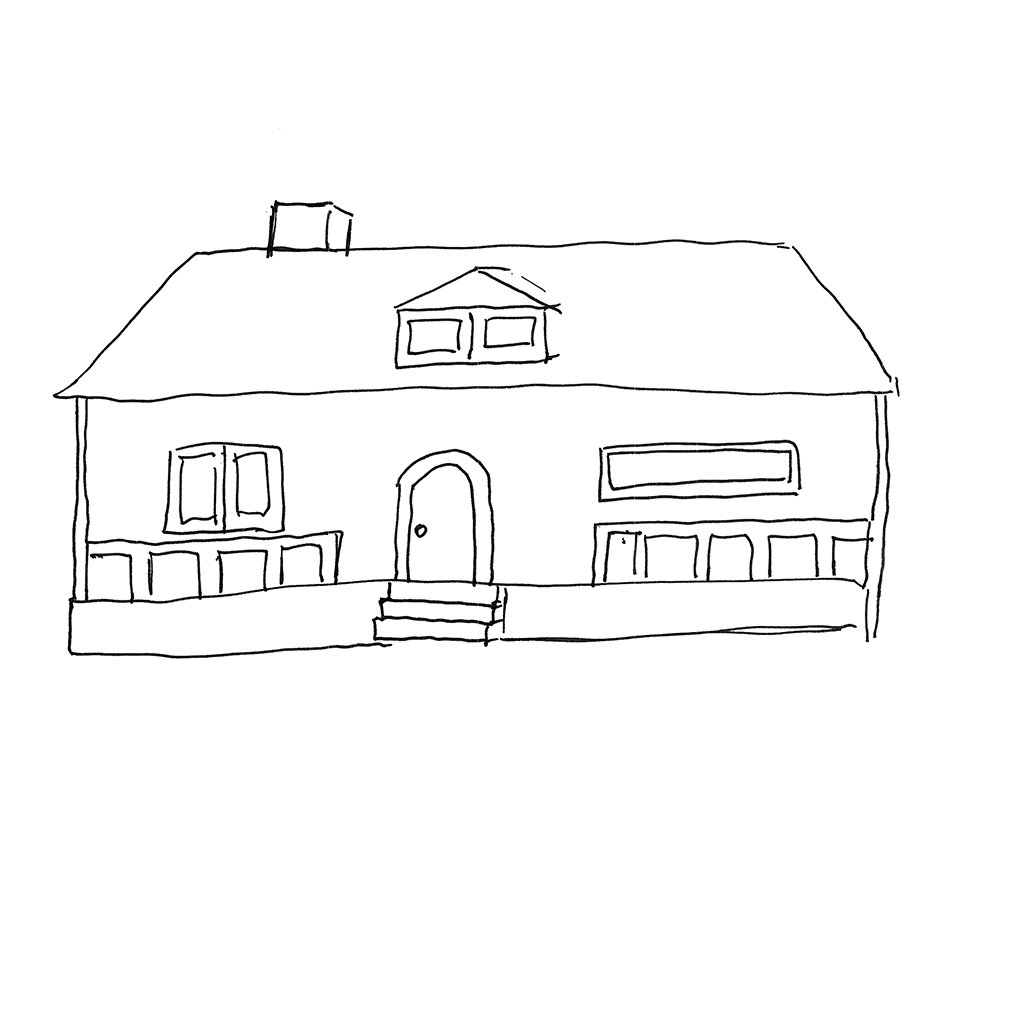
\includegraphics[width = 0.3\textwidth]{images/sketch2.jpg}}
\hspace{5mm}
\subfloat[]{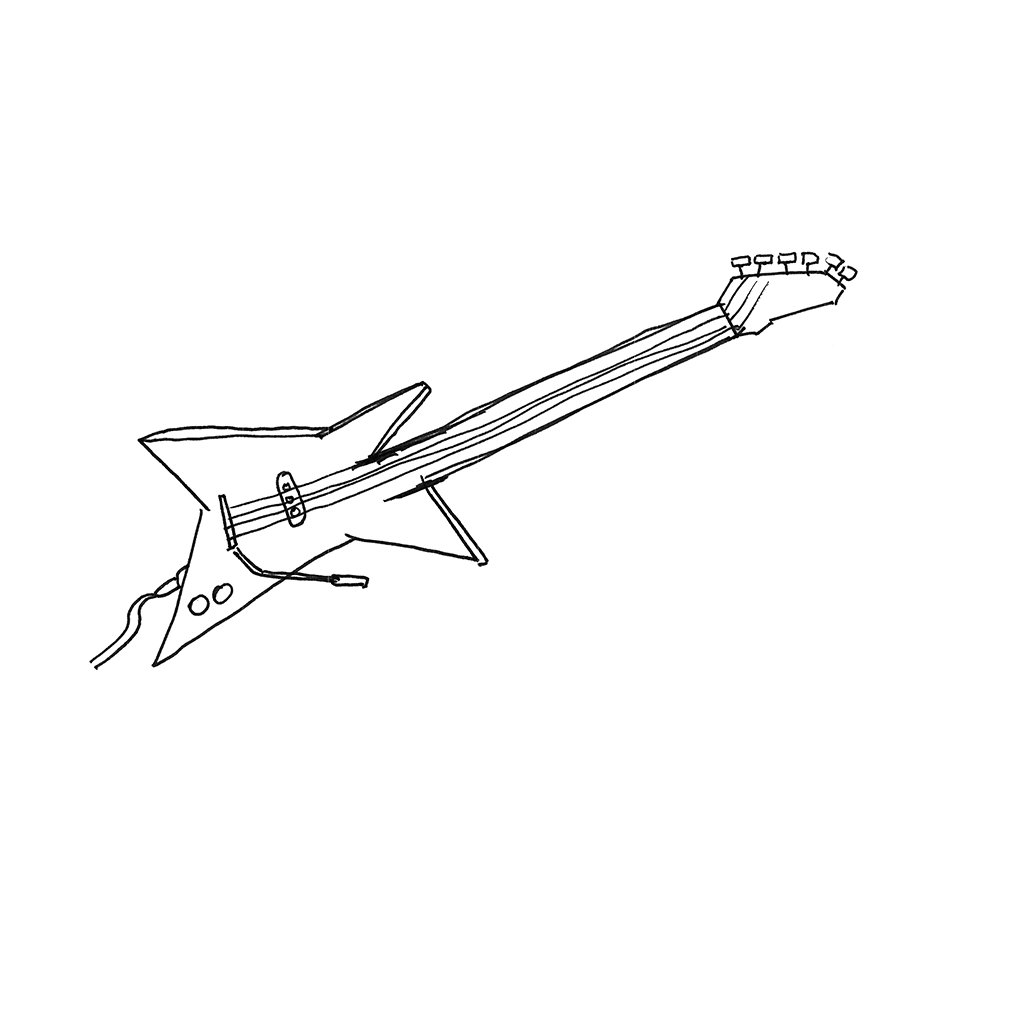
\includegraphics[width = 0.3\textwidth]{images/sketch3.jpg}}
\hspace{5mm}
\caption{sketches}
\label{fig:sketches}
\end{figure}


\begin{table}[H]
%\caption{single vs. cluster}
\centering
\begin{tabular}{| c c | c | c | c|}
\hline\hline
Image & bpp & SPRS & JPEG & JPEG2000 \\
\hline
a & 0.084 & 33.9594 & 28.9578 & 38.3258  \\
b & 0.13 & 32.9 & 34.5546 &  40.0159 \\
c & 0.08 & 32.5131 & 28.6558 & 36.3093  \\
\hline
\end{tabular}
\end{table}

\begin{figure}[H]
\centering
\subfloat[sprs]{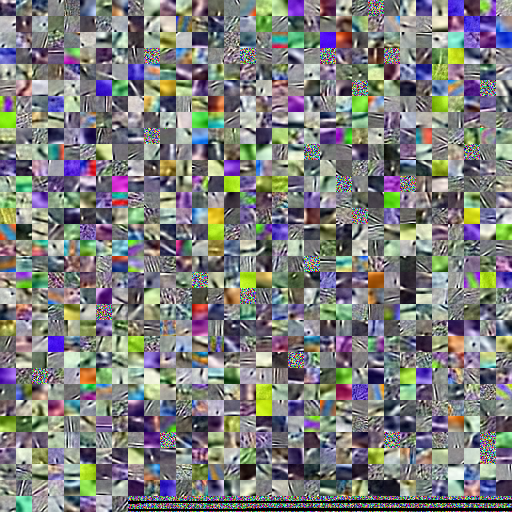
\includegraphics[width =
0.3\textwidth]{images/16_1000_1000_10_lasso.png}}
\hspace{5mm}
\subfloat[JPEG]{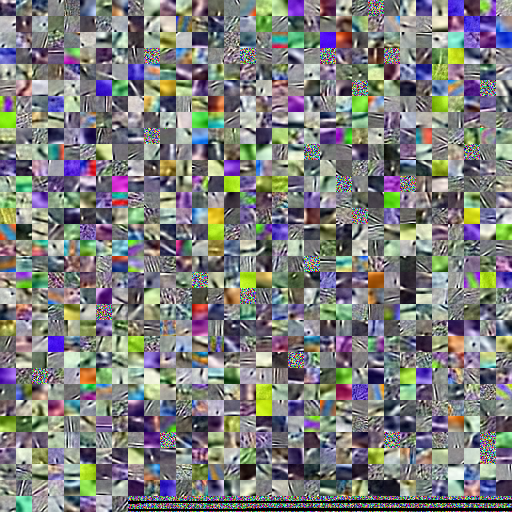
\includegraphics[width =
0.3\textwidth]{images/16_1000_1000_10_lasso.png}}
\hspace{5mm}
\subfloat[JPEG2000]{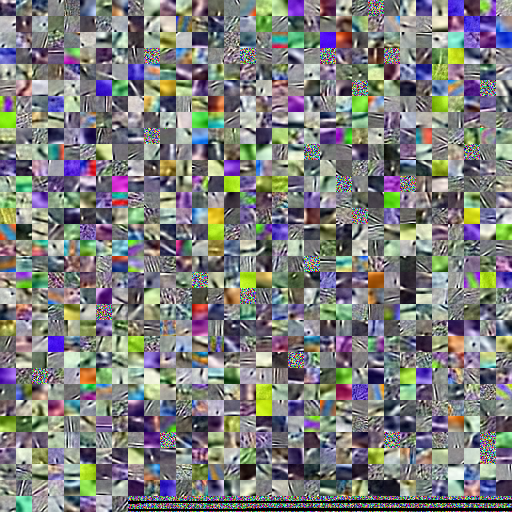
\includegraphics[width =
0.3\textwidth]{images/16_1000_1000_10_lasso.png}}
%\caption{}
%\label{fig:16_1000_lasso}
\end{figure}

\begin{figure}[H]
\centering
\subfloat[sprs]{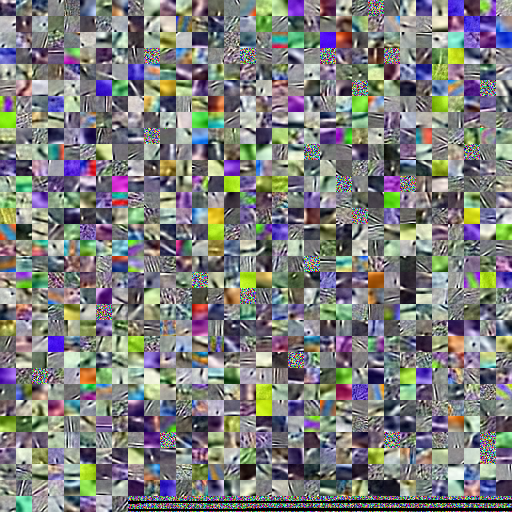
\includegraphics[width =
0.3\textwidth]{images/16_1000_1000_10_lasso.png}}
\hspace{5mm}
\subfloat[JPEG]{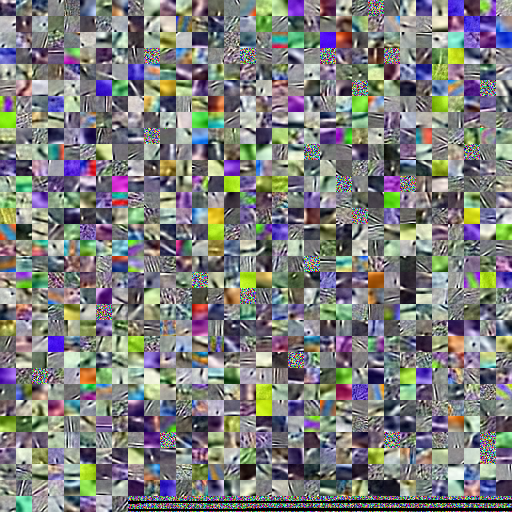
\includegraphics[width =
0.3\textwidth]{images/16_1000_1000_10_lasso.png}}
\hspace{5mm}
\subfloat[JPEG2000]{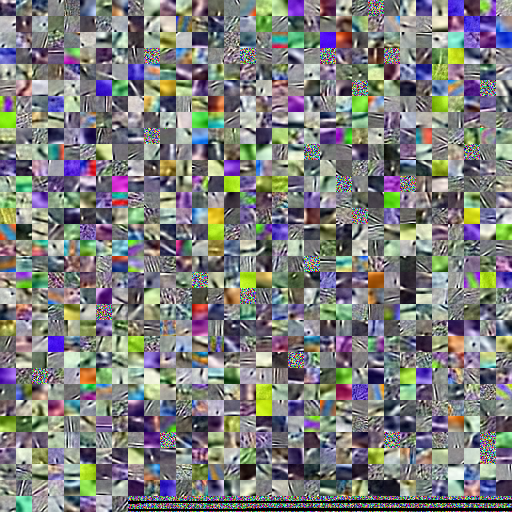
\includegraphics[width =
0.3\textwidth]{images/16_1000_1000_10_lasso.png}}
%\caption{}
%\label{fig:16_1000_lasso}
\end{figure}

% This chapter shows the results and discussion for the following experiments.
% % Reconstruction quality is mean of PSNR of images inside and outside of
% % the training sets.
% \begin{enumerate}
%  \item Convergence of reconstruction quality for different dictionary sizes.
%  \item Comparison of reconstruction quality of dictionaries
% in single and in cluster runs. 
%  \item Comparison of compression quality between learned dictionaries, JPEG
%and
% JPEG2000  on natural images and sketches.
%  \item Observations of structures of dictionary atoms from different
% groups of images and block sizes.
% \end{enumerate}









